% CogFormer — Encoder (set encoder -> summary tokens)
% Literal computational block diagram. Compile standalone:
%   pdflatex cogformer_encoder.tex
\documentclass[border=8pt]{standalone}
\usepackage{amsmath}
\usepackage{amssymb}
\usepackage{tikz}
\usetikzlibrary{arrows.meta, positioning, fit, backgrounds, calc}

\begin{document}
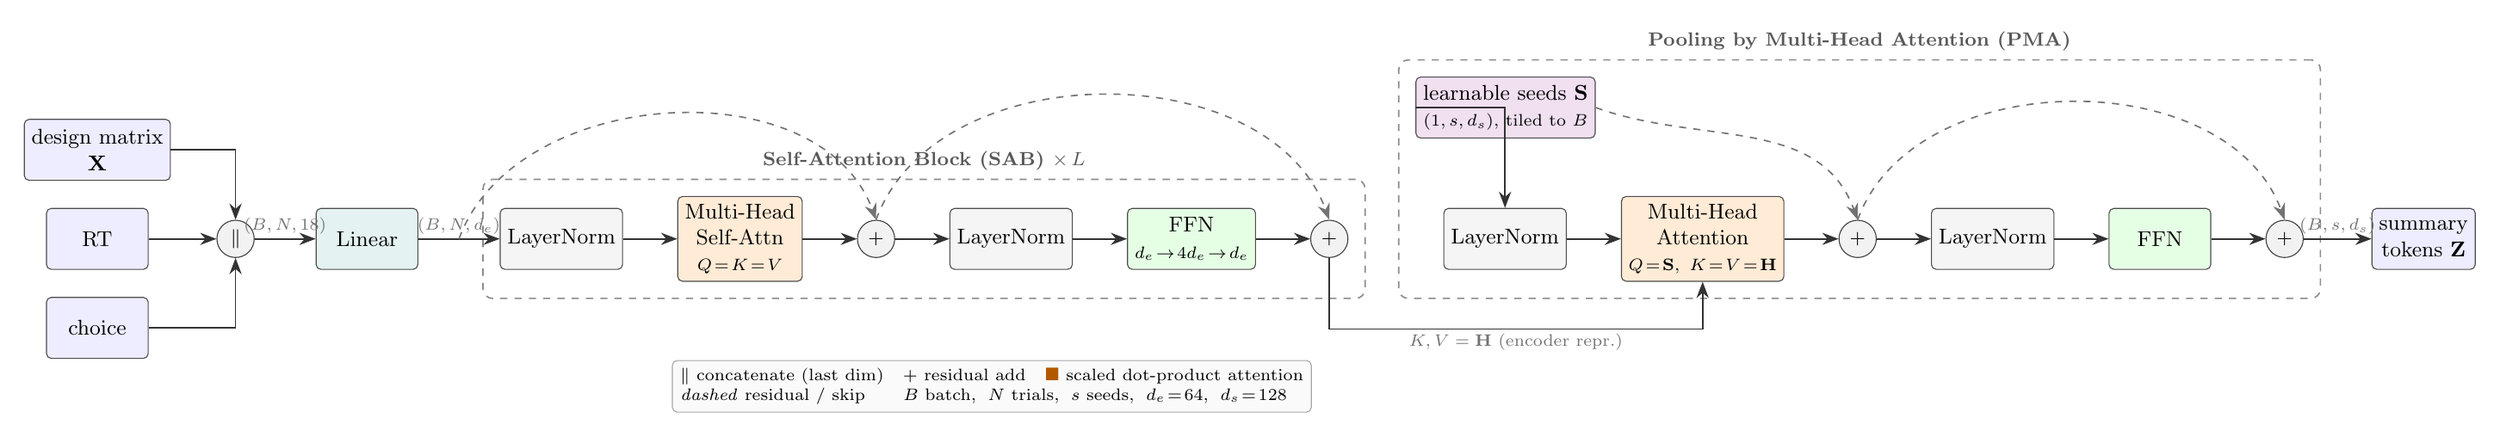
\begin{tikzpicture}[
  font=\small,
  node distance=8mm,
  >={Stealth[length=2.4mm]},
  block/.style={rounded corners=2pt, draw=black!70, fill=#1,
                minimum height=9mm, minimum width=15mm, align=center, inner sep=3pt},
  block/.default=white,
  data/.style={block=blue!7},
  lin/.style={block=teal!10},
  norm/.style={block=black!4, minimum width=12mm},
  attn/.style={block=orange!16, minimum height=12mm},
  ffn/.style={block=green!10},
  seed/.style={block=violet!12},
  op/.style={circle, draw=black!75, fill=black!5, inner sep=0pt,
             minimum size=5.5mm, font=\footnotesize},
  grp/.style={rounded corners=4pt, draw=black!45, dashed, line width=0.6pt, inner sep=7pt},
  grplab/.style={font=\footnotesize\bfseries, text=black!65},
  flow/.style={->, semithick, draw=black!80},
  res/.style={->, semithick, draw=black!55, dashed},
  shp/.style={font=\scriptsize, text=black!55, inner sep=1.5pt},
]

% ---------- Inputs ----------
\node[data] (x)  {design matrix\\$\mathbf{X}$};
\node[data, below=4mm of x]  (rt) {RT};
\node[data, below=4mm of rt] (ch) {choice};
\node[op, right=10mm of rt] (cat) {$\Vert$};
\draw[flow] (x)  -| (cat);
\draw[flow] (rt) -- (cat);
\draw[flow] (ch) -| (cat);

% ---------- Input embedding ----------
\node[lin, right=9mm of cat] (emb) {Linear};
\draw[flow] (cat) -- (emb) node[shp, midway, above]{$(B,N,18)$};

% ---------- Self-Attention Block (x L) ----------
\node[norm, right=12mm of emb] (sln1) {LayerNorm};
\node[attn, right=of sln1]     (smha) {Multi-Head\\Self-Attn\\{\scriptsize$Q\!=\!K\!=\!V$}};
\node[op,   right=of smha]     (sa1)  {$+$};
\node[norm, right=of sa1]      (sln2) {LayerNorm};
\node[ffn,  right=of sln2]     (sffn) {FFN\\{\scriptsize$d_e\!\to\!4d_e\!\to\!d_e$}};
\node[op,   right=of sffn]     (sa2)  {$+$};

\draw[flow] (emb) -- (sln1) node[shp, midway, above]{$(B,N,d_e)$};
\draw[flow] (sln1) -- (smha);
\draw[flow] (smha) -- (sa1);
\draw[flow] (sa1)  -- (sln2);
\draw[flow] (sln2) -- (sffn);
\draw[flow] (sffn) -- (sa2);
% residual connections (pre-LN)
\coordinate (stap) at ($(emb.east)!0.5!(sln1.west)$);
\draw[res] (stap) to[out=70,in=110] (sa1.north);
\draw[res] (sa1.north) to[out=70,in=110] (sa2.north);

\begin{scope}[on background layer]
  \node[grp, fit=(sln1)(smha)(sa1)(sln2)(sffn)(sa2),
        label={[grplab]above:Self-Attention Block (SAB) $\times\,L$}] (sabgrp) {};
\end{scope}

% ---------- Pooling by Multi-Head Attention ----------
\node[seed, above=12mm of sa2, xshift=26mm] (seed)
      {learnable seeds $\mathbf{S}$\\{\scriptsize$(1,s,d_s)$, tiled to $B$}};
\node[norm, right=14mm of sa2] (pln1) {LayerNorm};
\node[attn, right=of pln1]     (pmha) {Multi-Head\\Attention\\{\scriptsize$Q\!=\!\mathbf{S}$,\, $K\!=\!V\!=\!\mathbf{H}$}};
\node[op,   right=of pmha]     (pa1)  {$+$};
\node[norm, right=of pa1]      (pln2) {LayerNorm};
\node[ffn,  right=of pln2]     (pffn) {FFN};
\node[op,   right=of pffn]     (pa2)  {$+$};

\draw[flow] (seed) -| (pln1);
\draw[flow] (pln1) -- (pmha);
\draw[flow] (pmha) -- (pa1);
\draw[flow] (pa1)  -- (pln2);
\draw[flow] (pln2) -- (pffn);
\draw[flow] (pffn) -- (pa2);
% K,V come from the encoder representation H (= SAB output); route below the query LN
\draw[flow] (sa2.south) -- ++(0,-1.05) -| (pmha.south)
      node[shp, pos=0.25, below]{$K,V=\mathbf{H}$ (encoder repr.)};
% residuals on the seed/query stream
\draw[res] (seed.east) to[out=-20,in=110] (pa1.north);
\draw[res] (pa1.north) to[out=70,in=110] (pa2.north);

\begin{scope}[on background layer]
  \node[grp, fit=(pln1)(pmha)(pa1)(pln2)(pffn)(pa2)(seed),
        label={[grplab]above:Pooling by Multi-Head Attention (PMA)}] (pmagrp) {};
\end{scope}

% ---------- Output ----------
\node[data, right=10mm of pa2] (z) {summary\\tokens $\mathbf{Z}$};
\draw[flow] (pa2) -- (z) node[shp, midway, above]{$(B,s,d_s)$};

% ---------- Legend ----------
\node[draw=black!35, rounded corners=2pt, fill=black!2, align=left,
      font=\scriptsize, below=9mm of sabgrp.south, anchor=north, xshift=10mm] (leg)
  {$\Vert$ concatenate (last dim)\quad
   $+$ residual add\quad
   {\color{orange!70!black}$\blacksquare$} scaled dot-product attention\\
   \textit{dashed} residual / skip\qquad
   $B$ batch,\; $N$ trials,\; $s$ seeds,\; $d_e\!=\!64$,\; $d_s\!=\!128$};

\end{tikzpicture}
\end{document}
